% !TEX root = ./docs.tex


Test

Die Anwendung soll //TODO

Aus diesem Grund wird die Anwendung von mehreren Gleichwertigen Servern bedient. Jeder dieser sog. Nodes hat dabei eine vollständige Kopie sämtlicher dem System bekannten Daten. Eine Veränderung des Datenbestandes muss dem entsprechend an alle anderen Nodes weiter gegeben.

Jeder Client kann sich zu einer Node verbinden. Möchte dieser eine Nachricht an einen weiteren Client senden, schickt er diese an seine verbundene Node und überlässt die Zustellung dieser. Da alle Nachrichten aus Persitenzgründen an alle Nodes verteilt werden müssen, brauchen die Nodes keine Information über die Clients anderer Nodes. Im Falle einer solchen Anforderung (z.\,B. Abfrage ob ein anderer Nutzer aktiv ist) könnte ein Protokoll ähnlich zu Routing-Tabellen implementiert werden. Empfängt eine Node eine Nachricht, egal ob von einem Client oder von einer anderen Node, überprüft diese ob die Nachricht für einen ihr bekannten Client bestimmt war und sendet diese gegebenenfalls an diesen.

\begin{figure}[h]
    \centering
    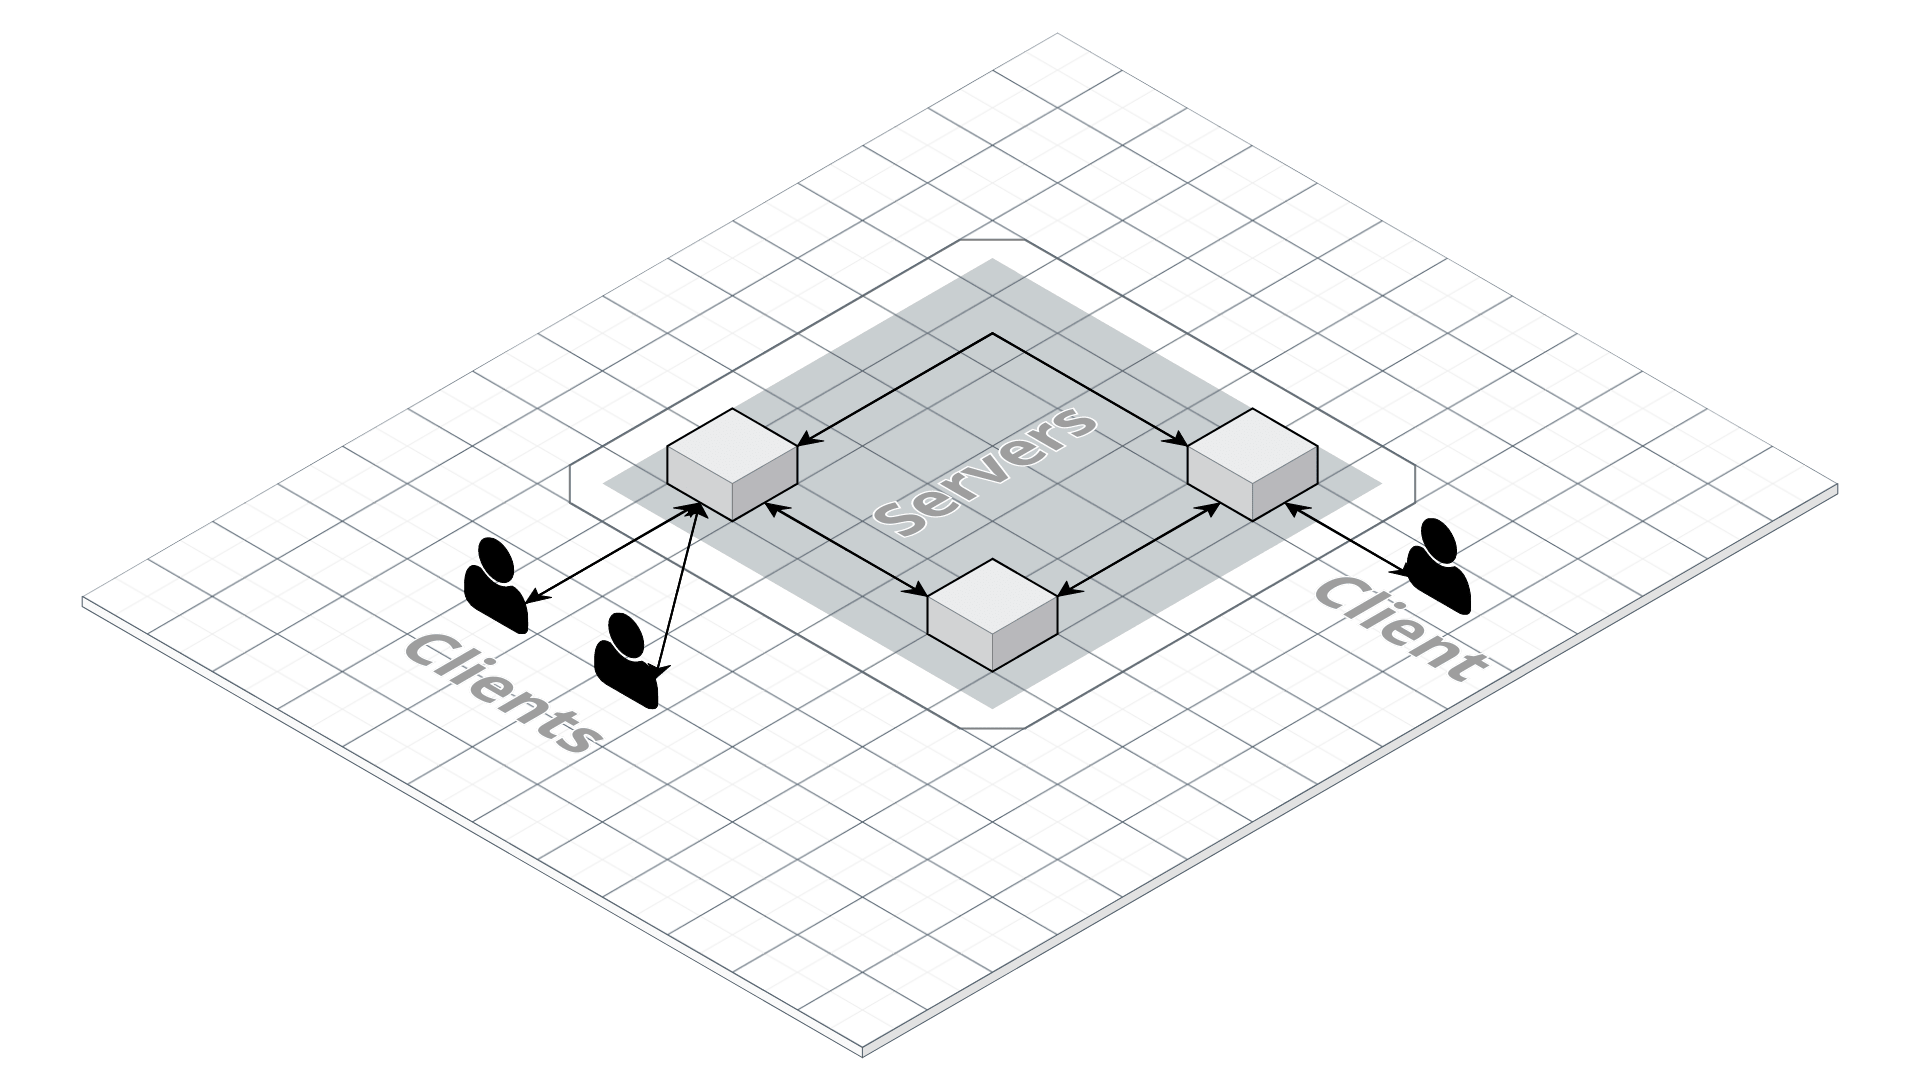
\includegraphics[width=\textwidth]{architecture.png}
    
    \caption{Architecture}
    \label{}
\end{figure}